\chapterimage{chapter_head_1.pdf} % Chapter heading image
\chapter{Dynamic programming}

\subsection{A. Gellyfish and Flaming peony}
\begin{sloppypar}
\url{https://codeforces.com/problemset/problem/2115/A} 
\end{sloppypar}

It can be shown that ultimately all elements become 
$$ G = \gcd(a_1, a_2, \ldots, a_n). $$
\begin{obs}
If there is an element \( a_k = G \), then all the other elements will become \( G \).  
We just need to count the number of elements where \( a_i \neq G \ \forall i \).
\end{obs}

But if initially \( G \notin a \), then we have to calculate the number of operations to make an element in \( a \) equal to \( G \).  
We can do this using dynamic programming,
$$ f(x) = \text{\# of operations to make an element in } a \text{ equal to } x. $$

the transition equation is
$$ f(\gcd(x, a_i)) = f(x) + 1 $$

computed \( \forall x \in [\max(a) \dots 1], \quad \forall i \in \{1, 2, \ldots, n\} \)  
by updating when we find a smaller value at every iteration.

In addition, \( \gcd(a, b) \) takes \( \log(a) \) time so we need to preprocess the \texttt{gcd} function to avoid the complexity. To compute the 2 nested \texttt{for} loops will take
\[
\mathcal{O}(n \cdot \max(a) \cdot \log(\max(a)))
\]

We create a matrix for which
$$ \gcd[x][y] = \gcd[y][x] = \gcd[y][x \bmod y] $$

and this takes \( \mathcal{O}(\max(a) \cdot n) \), but we have the constraints:  
$$ 1 \leq a_i, n \leq 5000, $$
so the complexity is really  
\[
\mathcal{O}(\max(a)^2) = \mathcal{O}(n^2), \quad \text{which will be at most } (5 \cdot 10^3)^2 = 25 \cdot 10^6 \text{ operations, which is acceptable.}
\]

Therefore, we would have:
\[
\begin{array}{c|c}
\textbf{Preprocessing} & \textbf{Per Test Case} \\
\hline
\mathcal{O}(\max(a)^2) = \mathcal{O}(n^2) & \mathcal{O}(n \cdot \max(a)) = \mathcal{O}(n^2)
\end{array}
\]
\[
= \mathcal{O}(n^2) + \mathcal{O}(n^2) = \mathcal{O}(n^2)
\]

You can visualize the solution as: there is a chain of operations you do that interconnects the elements in a, and to get to g you choose one of the chains.
If you visualize it so, there are a lot of paths to take, and we eventually could arrive at the same number \( x_k \) via different paths; but in general for a specific point you are in the chain, you want the minimum cost out of all the possible paths.

And how can you take all the good possible paths? \\
By enumerating all possible \( x \)'s and all possible \( a_i \)'s.

\begin{obs}
    We know $\gcd(x, a_i) \leq x$ hence the choice of enumerating x from $\max(a)$ to $1$. Because we first fill $f(x)$ and then we can use those values to fill $f(gcd(x, a_i))$.
\end{obs}


\begin{minted}{C++}
#include <bits/stdc++.h>
using namespace std;
using ll=long long;
#define debug(x) cout << #x << " = " << x << '\n';
#define vdebug(a) cout << #a << " = "; for(auto x: a) cout << x << " "; cout << '\n';
typedef vector<ll> vi;
typedef pair<ll, ll> pi;

#define N 5005
ll g[N][N];

void test_case() {
  ll n; cin >> n;
  vi a(n), f(N, LLONG_MAX / 2LL);
  ll mx = 0, k = 0; // mx = max(a), k = gcd(a[0], ... , a[n-1])

  for (ll &x : a) {
    cin >> x;
    k = g[k][x];
  }
  
  for (ll &x : a) {
    // x /= k;
    mx = max(mx, x);
    f[x] = 0;
  } 
  
  for (ll x = mx; x >= 1; x--) {
    for (ll &y : a) {
      // remember that we want to minimize the number of operations
      if (f[g[x][y]] > f[x] + 1)
        f[g[x][y]] = f[x] + 1;
    }
  }
  
  ll ans = max(f[k] - 1, 0LL);
  for (ll &x : a) 
    if (x > k) ans++;

  cout << ans << endl;
}

int32_t main() {
  ios_base::sync_with_stdio(0); cin.tie(0);

  for (ll i=0; i<N; i++) g[i][0] = g[0][i] = g[i][i] = i;
  for (ll x=1; x<N; x++) {
    for (ll y=1; y<x; y++) {
      g[x][y] = g[y][x] = g[y][x % y];
    }
  }

  int t;
  cin >> t;
  while (t--) {
    test_case();    
  }
}
\end{minted}

\subsection{Book shop}
\begin{sloppypar}
\url{https://cses.fi/problemset/task/1158}
\end{sloppypar}

This problem is equivalent to the classical \textbf{knapsack problem}. This problem comes down to analysing 2 cases only:
\\
\begin{itemize}
    \item \textbf{Excluding the $i$-th item}, in which case the best solution is the same as the one obtained by considering only the items with indices from $1$ to $i - 1$;
    
    \item \textbf{Including the $i$-th item}, in which case the best solution is obtained by using $h_i$ units of capacity for the new item, and optimally using the remaining $j - h_i$ units of capacity for the previous items.
\end{itemize}


\begin{center}
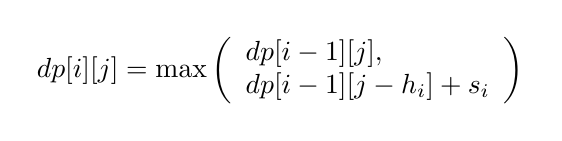
\begin{tikzpicture}[every node/.style={font=\normalsize}]
    % Main DP formula
    \node (dp) at (0,0) {$
        \text{dp}[i][j] = \max\left(
            \begin{array}{l}
                \text{dp}[i - 1][j], \\
                \text{dp}[i - 1][j - h_i] + s_i
            \end{array}
        \right)
    $};
\end{tikzpicture}
\end{center}

where we define dp[$i$][$j$] as the maximum number of pages we can buy with $j$ dollars and including all the books from $1$ to $i$.


\subsection{Counting Towers}
\begin{sloppypar}
\url{https://cses.fi/problemset/task/2413}
\end{sloppypar}

We distinguish between type 1 towers, and type 2. Type 1 towers have the the top two cells connected, while type 2 towers have the top two cells that are part of different blocks.

\begin{figure}[!ht]
    \centering
    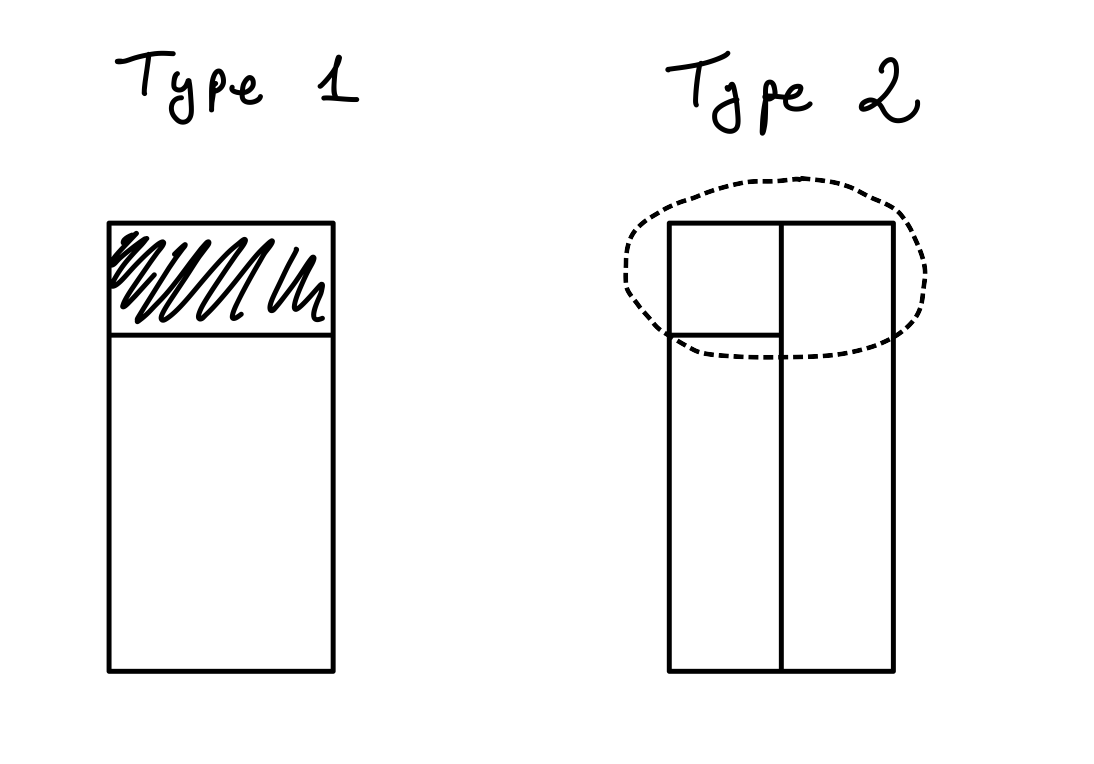
\includegraphics[width=0.5\linewidth]{Pictures/2-1.png}
    \caption{2 types of towers}
    \label{fig:21}
\end{figure}

We let $a_n$ = no. of towers of type 1 of height $n$, $b_n$ = no. of towers of type 2 of height $n$.

\begin{figure}[!ht]
    \centering
    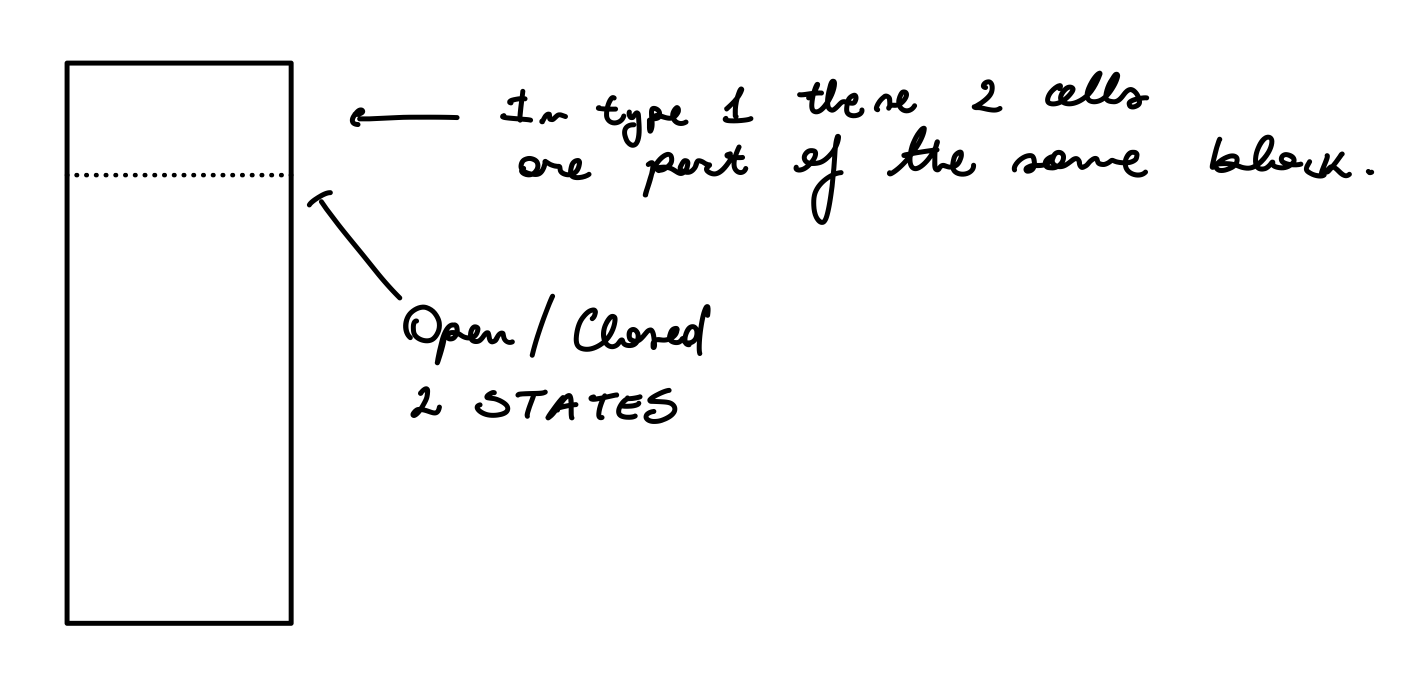
\includegraphics[width=0.75\linewidth]{Pictures/2-2.png}
    \caption{We can view the line below the $i$-th row as open or closed.}
    \label{fig:22}
\end{figure}

\subsubsection{Type 1 towers}
If we have the top 2 cells connected ($i$-th row) the dotted line (Figure \ref{fig:22}) could be empty or filled and then below it we either put a tower $(i - 1) \times 2$ of type 1. Otherwise the dotted line is filled and then we put a tower $(i - 1) \times 2$ of type 2.

\begin{equation}
    a_n = 2a_{n-1} + b_{n-1}
\end{equation}

\subsubsection{Type 2 towers}
For a type 2 tower we have a line that splits vertically the top 2 cells (see figure \ref{fig:21}) and the dotted line show in figure \ref{fig:22} can be either filled or open, leading to \textbf{4 possible states}. Below this line we could fill with type 2 towers. If we want to fill the remaining spaces with a type 1 tower we have to account for the fact that its top two cells have to be part of the same block, so the dotted line is \textit{filled}. This leads to only \textbf{1 possible state}.

\begin{equation}
    b_n = 4b_{n-1} + a_{n-1}
\end{equation}

The number of towers is $a_n + b_n$. We simply compute every value of $a_i, b_i$ leading to a complexity of $O(n)$.

\begin{minted}{c++}
#include <bits/stdc++.h>
using namespace std;
using ll=long long;
#define debug(x) cout << #x << " = " << x << '\n';
#define vdebug(a) cout << #a << " = "; for(auto x: a) cout << x << " "; cout << '\n';
typedef vector<ll> vi;
typedef pair<ll, ll> pi;

const ll mod = 1e9 + 7;

void test_case() {
  ll n; cin >> n; 
  
  ll a = 1, b = 1;
  if (n == 0) cout << "0\n";
  else if (n == 1) cout << "2\n";
  else {
    for (ll i = 2; i <= n; i++) {
      ll newa = (2*a + b) % mod;
      ll newb = (4*b + a) % mod;
  
      a = newa, b = newb;
    }
  
    cout << (a + b) % mod << endl;
  }
}
\end{minted}

\section{Constructing permutations and combinations}

\subsection{Coin combinations I \&\& II: swapping two loops can change the result!}
\begin{sloppypar}
\url{https://cses.fi/problemset/task/1635}, \url{https://cses.fi/problemset/task/1636} 
\end{sloppypar}

\subsubsection{Coin combinations I}
The first problem asks us to calculate all the distinct \textit{permutations} of a set of coins to produce a certain sum of money $x$. 
\begin{equation}
    \text{dp}[i] = \text{\# of permutations of coins that sum up to amount } i.
\end{equation}

\begin{minted}{c++}
void test_case() {
  ll n, x; cin >> n >> x;
  vector<ll> c(n);
  vector<ll> dp(x+1, 0);
  for (auto &x : c) cin >> x;

  dp[0] = 1;

  for (ll i = 1; i <= x; i++) {
    for (ll coin : c) {
      if (i - coin >= 0)
        dp[i] += (dp[i - coin] % mod);
    }
  }
  
  cout << (dp[x] % mod) << endl;
}

\end{minted}

The approach we take is iterating through the amounts $i$ ($1 \leq i \leq x$) and then trying all the possible coins to make that amount. If we want to make amount $i$, there are $\text{dp}[i - c]$ ways of doing that, where $c$ is a coin in the set that we use to complete the permutation. 
That is we are constructing all the permutations of this kind,

\begin{equation}
    (c, (\text{all the permutations that sum up to } i - c \text{ go here}))
\end{equation}


\subsubsection{Coin combinations II}

Here what's asked is to count the number of \textit{combinations} to make an amount $x$ with a given input set of coins. 

The approach we take is to select a coin $c$, and from here compute
\begin{equation}
    \text{dp}[i] = \text{\# of combinations using the given coins to reach amount } i, \forall i\ (1 \leq i \leq x). 
\end{equation}


\begin{idea}
    Here adding $3 + 1$ is the same as adding $1 + 3$, this means that we need to consider the coins in order. So we only go through the set of coins once, thus it's impossible to create two combinations with the same set of coins ordered differently. This is different from the previous problem where we considered every coin at all times.
\end{idea}

We get a time complexity of $\mathcal{O}(n \cdot x)$.

\begin{minted}{c++}
void test_case() {
  ll n, x; cin >> n >> x;
  vector<ll> c(n);
  vector<ll> dp(x+1, 0);
  for (auto &x : c) cin >> x;

  dp[0] = 1;

  for (ll coin : c) {
    for (ll i = 1; i <= x; i++) {
      if (i - coin >= 0)
        dp[i] += (dp[i - coin] % mod);
    }
  }
  
  cout << (dp[x] % mod) << endl;
}
\end{minted}

At every iteration of the outer loop we add a coin to the ones that we are using in order to construct the combinations. That is, at the first iteration we are calculating how to make all the possible amounts $1 \leq i \leq x$ only using the first coin. At the second iteration only using the first two coins, and so forth.

This means that we could have done the same job using a matrix instead of iterating on the same array multiple times by defining
\begin{equation}
    \text{dp}[j][i] = \text{\# of combinations to produce a sum of money $i$ using the first $j$ coins}.
\end{equation}

\subsection{Dice Sum}
\url{https://atcoder.jp/contests/abc248/tasks/abc248_c} \\ 

We want to construct all the permutations of this kind,
\begin{equation}
    (A_1, \dots, A_n)
\end{equation}

where $A_i \in [1 \dots M]$ and $\sum_{1 \leq i\leq N}{A_i} \leq K$.

What we do is again, as we did in Coin Combinations I, first try to put a number $A_1$ and then construct sum the amount of permutations that have length $n - 1$. 

\begin{minted}{c++}
#include <bits/stdc++.h>
using namespace std;
using ll=long long;
#define debug(x) cout << #x << " = " << x << '\n';
#define vdebug(a) cout << #a << " = "; for(auto x: a) cout << x << " "; cout << '\n';
typedef vector<ll> vi;
typedef pair<ll, ll> pi;

const ll mod = 998244353LL;

void test_case() {
  ll N, M, K; cin >> N >> M >> K;

  // dp[i][k] = # of sequences of length i and sum = k.
  vector<vi> dp(N+1, vi(K+1));

  for (ll k = 1; k <= K; k++) {
    if (k <= M)
      dp[1][k] = 1;
  }

  for (ll i = 1; i <= min(N, K); i++)
    dp[i][i] = 1;
  
  for (ll i = 2; i <= N; i++) { // len
    for (ll k = i+1; k <= K; k++) { // sum

      for (ll p = 1; p <= M; p++) {
        if (k - p >= 1)
          dp[i][k] += (dp[i-1][k - p] % mod);
      }

    }
  }

  // sequences of len N where sum <= K
  cout << accumulate(dp.back().begin(), dp.back().end(), 0LL) % mod << endl;
}

int32_t main() {
  ios_base::sync_with_stdio(0); cin.tie(0);
  test_case();
}
\end{minted}
